
%figurstørrelser.

\documentclass[english,notitlepage]{revtex4-1}  % defines the basic parameters of the document
% if you want a single-column, remove reprint

% allows special characters (including æøå)
\usepackage[utf8]{inputenc}
\usepackage [norsk]{babel} %if you write norwegian
%\usepackage[english]{babel}  %if you write english


%% note that you may need to download some of these packages manually, it depends on your setup.
%% I recommend downloading TeXMaker, because it includes a large library of the most common packages.

\usepackage{physics,amssymb}  % mathematical symbols (physics imports amsmath)
\usepackage{graphicx}         % include graphics such as plots
\usepackage{xcolor}           % set colors
\usepackage{hyperref}         % automagic cross-referencing (this is GODLIKE)
\usepackage{tikz}             % draw figures manually
\usepackage{listings}         % display code
\usepackage{subfigure}        % imports a lot of cool and useful figure commands
\usepackage{verbatim}

% defines the color of hyperref objects
% Blending two colors:  blue!80!black  =  80% blue and 20% black
\hypersetup{ % this is just my personal choice, feel free to change things
    colorlinks,
    linkcolor={red!50!black},
    citecolor={blue!50!black},
    urlcolor={blue!80!black}}

%% Defines the style of the programming listing
%% This is actually my personal template, go ahead and change stuff if you want
\lstset{ %
	inputpath=,
	backgroundcolor=\color{white!88!black},
	basicstyle={\ttfamily\scriptsize},
	commentstyle=\color{magenta},
	language=Python,
	morekeywords={True,False},
	tabsize=4,
	stringstyle=\color{green!55!black},
	frame=single,
	keywordstyle=\color{blue},
	showstringspaces=false,
	columns=fullflexible,
	keepspaces=true}

\begin{document}



\title{Oppgave 1C.4: Ekstrasolare planeter}
\date{\today}
\author{Knadidatnr.: 15889}
\affiliation{Institute of Theoretical Astrophysics, University of Oslo}
\email{textme@astro.uio.no}


\newpage

\begin{abstract}
Jeg har studert måledata for bølgelengde og fluks til lys som når oss fra fem fjerne
 stjerner. Siden lyset blir rød- og blåforskjøvet på grunn av Doppler-effekten var jeg i stand til å finne hastighetene som disse stjernene beveger seg med i forhold til oss, og for flere av stjernene, hvilke hastigheter de har i banene sine rundt et massesenter for solsystemet. Stjerner som går i bane rundt et massesenter må være påvirket av gravitasjonskrefter fra en eller flere planeter. Jeg har på den måten kunnet påvise planeter i bane rundt tre av stjernene. Ved hjelp av minste kvadraters metode har jeg funnet verdier for parametre som beskriver stjernenes bevegelse, og ved hjelp av disse produsert gode estimater for massen til to av disse planetene. Planetene har masse 2.9 og 5.1 ganger så store som Jupiter. Disse tallene er funnet ved hjelp av uttrykk utledet fra Keplers og Newtons lover. Jeg var ikke i stand til å si noe om radius eller atmosfære til planetene fordi det var for lang tid mellom målingene i dataen. Metoder er beskrevet som kan la oss finne radius til planeter i tillegg til størrelse og innhold i deres atmosfære dersom vi har tilgang til tilstrekkelig måledata. 


\end{abstract}
\maketitle                                % creates the title, author, date & abstract



\section{Introduksjon}
\label{sect:intro}

I dette prosjektet skal jeg studere lys som er observert fra fem fjerne stjerner. Målet
 er å lære så mye som mulig om disse stjernene og eventuelle planeter som går i bane rundt dem. Jeg håper å kunne finne ut hvor stor hastighet stjernene har i forhold til oss på jorda, og hvilke hastigheter stjernene og eventuelle planeter har i sine baner rundt deres felles massesenter. Med litt flaks kan vi også finne ganske eksakte verdier for massen og radien til planeter som går i bane rundt stjernene, og størrelse og innhold i atmosfæren.

Alt vi kan måle fra fjerne solsystemer og galakser er egenskaper ved den
 elektromagnetiske strålingen vi mottar fra dem. Å utvikle teorien og teknologien som brukes til å studere denne strålingen er er en avgjørende del av innsatsen som må legges ned for å øke vår forståelse av den delen av universet som ligger utenfor vår egen atmosfære. Dette prosjektet utforsker hva som er mulig å lære om stjerner og planeter som ligger langt unna vårt eget solsystem. Med de metoder som er beskrevet her kan man lære om bevegelsen til stjernene, finne radius og masse til eventuelle planeter som går i bane rundt dem, og til og med størrelse og innhold i atmosfæren til planetene. Dette er viktig for å påvise eksistensen av planeter utenfor vårt eget solsystem, og for å bestemme hvilke av disse planetene som har de nødvendige betingelsene for å støtte liv.


\section{Teori}

Ved å observere lyset som når oss fra fjerne stjerner kan vi finne ut hvilken fart
 stjernen har i forhold til oss her på jorda. På grunn av Doppler-Effekten vil lys sendt ut fra en kilde som beveger seg bort fra oss bli rødforskjøvet og lys fra en kilde som beveger seg mot oss vil bli blåforskjøvet. Likning \ref{eq:doppler} forteller oss hvordan vi kan finne hastigheten til lyskilden relativt til oss:

\begin{equation}
  \label{eq:doppler}
  \frac{\lambda - \lambda_0}{\lambda_0} = \frac{v_r}{c}
\end{equation}
der $\lambda$ er bølgelengden til det observerte lyset og $\lambda_0$ er bølgelengden vi
 måler for det samme lyset i laboratoriet på jorda. $v_r$ er farten til stjerna i forhold til oss og $c$ er lysfarten. Negativt fortegn på $v$ betyr at lyskilden er på vei mot oss, positivt fortegn betyr at den er på vei bort fra oss.

Som en forenklet problemstilling kan vi se på et system med en stjerne og en planet hvis
 massesenter beveger seg fra oss med en \textit{pekuliær} hastighet $v_{pec}$. På grunn av gravitasjonskreftene mellom de to legemene vil de begge bevege seg i ellipsebaner rundt et felles massesenter. Vi regner med at ellipsebanene er tilnærmet sirkulære, det betyr at stjernen og planeten begever seg med konstant banefart. Etterhvert som stjernen er på forskjellige punkter i sin bane rundt massesenteret vil vi observere at den har en hastighet som er ulik hastigheten til massesenteret. Den minste og største verdien vi måler for hastigheten får vi når stjernen beveger seg parallelt med massesenteret. Ved å se på differansen mellom farten til stjernen og farten til massesenteret kan vi finne banefarten til planeten rundt massesenteret. For å finne eksakte verdier må vi også ta hensyn til vinklingen til planetens bane i forhold til vår siktlinje. I tillegg vil vi på grunn av atmosfæriske forstyrrelser oppleve støy i målingene. For å finne de reelle verdiene for den dataen vi prøver å måle må vi fjerne denne støyen. Et plot av de observerte hastighetene kan se ut slik som i figur \ref{fig:theoretical_star_vel}.

\begin{figure}
  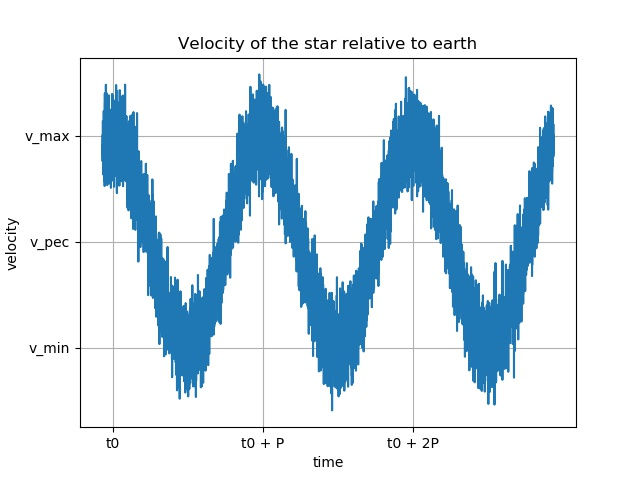
\includegraphics[width=\linewidth]{../output/plots/theoretical_star_vel.jpg}
  \caption{Hastigheten til en stjerne over en gitt tidsperiode. Hastigheten til massesenteret til systemet som består av planeten og stjernen, $v_{pec}$ er avmerket. Avmerket er også den største og den minste verdien vi observerer for farten til stjernen, $v_{max}$ og $v_{min}$. I tillegg til de reelle verdiene har vi støy som gjør at de reelle verdiene er vanskelige å avlese.}
  \label{fig:theoretical_star_vel}
\end{figure}

Når vi kjenner den maksimale radielle hastigheten til en stjerne, massen til stjernen og
 perioden i stjernens bane, kan vi finne en minsteverdi for massen til planeten som går i bane rundt stjernen. Utledningen baserer seg på Newtons og Keplers lover og forutsetter at massen til planeten $m_p$ er liten i forhold til massen til stjernen $m_\star$, slik at $1 + \frac{m_\star}{m_p} \approx \frac{m_\star}{m_p}$. Den fulle utledningen finnes i \citep{part1C}.

\begin{equation*}
  m_p \sin{i} = \frac{m_\star^{2/3} v_{\star r} P^{1/3}}{(2 \pi G)^{1/3}}
\end{equation*}
\begin{equation}
  \label{eq:planet_mass}
  m_p = \frac{m_\star^{2/3} v_{\star r} P^{1/3}}{(2 \pi G)^{1/3} \sin{i}} \geq \frac{m_\star^{2/3} v_{\star r} P^{1/3}}{(2 \pi G)^{1/3}}
\end{equation}

Her er $m_p$ massen til planeten, $i$ er vinkelen mellom vår siktlinje og normalvektoren
 til baneplanet, $m_\star$ er massen til stjernen, $v_{\star r}$ er den radielle komponenten til stjernens banehastighet, $P$ er perioden til stjernens banebevegelse og $G$ er gravitasjonskonstanten. Vinkelen $i$ er alltid mellom $0^\circ$ og $90^\circ$. $i$ er ikke kjent for oss, men ved å bruke likning \ref{eq:planet_mass} kan vi finne et tall for den minste massen planeten kan ha. For $i = 90^\circ$ er dette den virkelige massen til planeten.

Figur \ref{fig:theoretical_star_vel_nonoise} viser det samme som figur
 \ref{fig:theoretical_star_vel} uten støy. En matematisk modell som beskriver den radielle farten som funksjon av tid kan skrives på formen
 \begin{equation}
   \label{eq:v_model}
   v_r^{model} (t) = v_r \cos{\left( \frac{2 \pi}{P} (t - t_0) \right)}
 \end{equation}
 der $v_r$ er den maksimale verdien vi måler for farten, $P$ er perioden og $t_0$ er t-verdien for den første bølgetoppen. Vi ser at maksverdiene til funksjonen er $v_r^{model} (t = t_0 + iP) = v_r$ når $i$ er et heltall.

\begin{figure}
  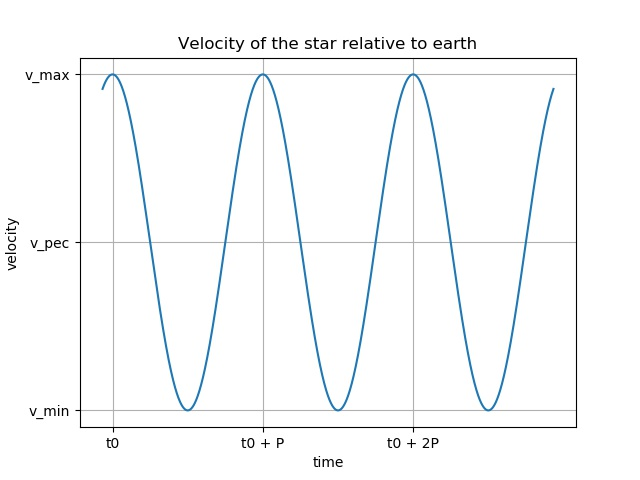
\includegraphics[width=\linewidth]{../output/plots/theoretical_star_vel_nonoise.jpg}
  \caption{Farten til en fjern stjerne sett fra jorda. Figuren viser det samme som figur \ref{fig:theoretical_star_vel}, men uten støy i målingene.}
  \label{fig:theoretical_star_vel_nonoise}
\end{figure}



\section{Metode}

Jeg har måledata fra fem forskjellige stjerner. Det jeg har tilgang til er bølgelengden
 til observert lys som i laboratoriet har en kjent bølgelengde $\lambda_0$ og fluksen til stjernen relativt til den maksimale fluksen for den gitte stjernen. For å finne farten til stjernen i forhold til oss kan vi løse likning \ref{eq:doppler} for $v_r$.

\begin{equation}
  \label{eq:v_r}
  v_r = \frac{\lambda - \lambda_0}{\lambda_0} c
\end{equation}

Ved å anvende likning \ref{eq:v_r} kan vi finne farten til hver av stjernene relativt til
 oss i alle tidssteg. For å finne pekuliærhastigheten til stjernen holder det å ta gjennomsnittet av alle de observerte verdiene for hastigheten. Stjernens hastighet varierer periodisk mellom $v_{min}$ og $v_{max}$, og gjennomsnittet vil ligge nært $v_{pec}$ når vi har mange jevnt fordelte målinger over et heltalls antall perioder. Se figur \ref{fig:theoretical_star_vel}. Jeg antar at støyen er normalfordelt med middelverdi 0. Da trenger jeg her ikke å ta hensyn til støyen når jeg beregner pekuliærhastigheten fordi støyen vil gi både positive og negative bidrag til middelverdien. Disse bidragene fra støyen vil etterhvert kansellere hverandre, og vi ender opp med den relle verdien for pekuliærhastigheten. Pekuliærhastigheten til en av stjernene er derfor bare middelverdien av alle de observerte hastigheten til stjerna i forhold til jorda.

For å finne ut mer om stjernene og eventuelle planeter som går i bane rundt dem, studerer
 jeg videre banene til stjernene. Den komponenten av banehastigheten til stjerne som er parallell med vår siktlinje kan vi finne ved å trekke pekuliærhastigheten fra den observerte hastigheten til stjerna. Da får vi en graf med samme form som \ref{fig:theoretical_star_vel}, som altså viser den radielle hastigheten til en stjerne i sin bane. Vi kan nå ved øyemål finne tilnærmede
 verdier for den maksimale radielle hastigheten til stjernene og perioden til
 hastighetskurven. For å finne maksimal fart ser man på funksjonsverdien til en bølgetopp
 i hastighetsplottet. Man må se gjennom støyen, og siden vi antar at støyen er
 normalfordelt med middelverdi 0, regner jeg den relle verdien som midtpunktet i det
 fargede området for en gitt t-verdi. På figur \ref{fig:theoretical_star_vel} kan man se
 at $v_{max}$ ligger midt i det fargede området for $t = t_0 + i*P$, der $i$ er et heltall. Perioden er avstanden langs tids-aksen mellom to punkter på grafen som svinger i samme fase, for eksempel mellom to bølgetopper.

Likning \ref{eq:planet_mass} gir oss nå en minsteverdi for massen til planeten som går i
 bane rundt en stjerne. For å beregne radien til en planet som passerer foran en stjerne kan vi se på hvor lang tid det går fra planeten begynner å bevege seg foran stjernen til hele planeten er mellom oss og stjernen. Fra den begynner å bevege seg foran stjernen vil fluksen vi måler fra stjernen bli redusert ettersom mer og mer av lyset blir blokkert av planeten. Mens hele planeten er foran stjernen vil vi måle en konstant verdi for fluksen som er mindre enn den verdien vi måler når planeten ikke er foran stjernen. Vi kan dermed se hvor lang tid det går fra planeten begynner å bevege seg foran stjernen til hele planeten er foran stjernen. Når vi også kjenner massen, og banefarten til stjernen og massen til planeten kan vi finne hastigheten til planeten i sin bane. Når vi kjenner tiden og hastigheten, kan vi finne hvor langt planeten har beveget seg i forhold til stjernen. Dette vil da være 2 ganger radien til planeten i løpet av den tiden det tar fra planeten begynner å bevege seg foran stjernen til hele planeten er foran stjernen. Dersom vi har tilgang til fluksen for lys av en annen bølgelengde kan det hende at vi kan finne størrelsen til en eventuell atmosfære på planeten og si noen om innholdet i den. Hvis fluksen reduseres mer for lys av en bestemt bølgelengde enn for annet lys, betyr det at et større areal blokkeres enn det som dekkes av selve planeten. Atmosfæren slipper gjennom lys med de fleste bølgelengder, men absorberer for noen bestemte frekvenser avhengig av hvilke stoffer som finnes i atmosfæren. Vi kan for eksempel se spor av vanndamp ved å observere at mer av lyset med bølgelengde som svarer til spektrallinjene til vanndamp er borte enn annet lys.

For å finne mer riktige verdier for hastigheten og perioden til stjernen og dermed også
 massen til eventuelle planeter som går i bane rundt den kan vi bruke uttrykket for $v_r^{model}$ (likning \ref{eq:v_model}). Vi ønsker å finne det beste estimatet for de ukjente parametrene $v_r$, $P$ og $t_0$ slik at funksjonen beskriver bevegelsen til stjernen best mulig. Det jeg ønsker å gjøre er å prøve modellen med mange forskjellige kombinasjoner av ulike verdier for disse parametrene og finne den kombinsjonen som gjør at modellen passer best med måledataen vi har tilgang til. Disse verdiene vil være mer nøyaktige enn de verdiene vi klarer å lese av med øyemål, og vil dermed kunne gi et mer nøyaktig estimat for massen til planeten. For å finne fram til disse verdiene velger jeg en øvre og nedre grense for hver av parametrene slik at jeg er sikker på at den verdien jeg er ute etter ligger innenfor intervallet. Deretter tester jeg modellen med 40 jevnt fordelte verdier innenfor dette intervallet, og plukker ut det settet med verdier som gir best tilnærming.

For å finne øvre og nedre grense for intervallene til parametrene bruker jeg en
 automatisk algoritme. Jeg observerer at måledataen for alle stjernene er registrert over ca. 2 perioder i stjernens bevegelse. Det vil si at perioden vil ligge et sted rundt halvparten av tidsforskjellen mellom den første og siste målingen. Ved å legge til en passende buffer på begge sider av denne verdien finner vi et intervall der vi kan teste ulike verdier for perioden. $t_0$ er tidspunktet for en bølgetopp (det spiller ingen rolle hvilken). Siden støyen er normalfordelt med middelverdi 0 og samme standardavvik hele tiden, kan vi anta at den største målte verdien for $v$ ligger i nærheten av den reelle maksverdien. Jeg legger derfor intervallet for hastigheten slik at tidspunktet for den største målte verdien av $v$ ligger i midten. For å finne den reelle maksverdien for observert hastighet tar jeg først gjennomsnittet av de 10 største verdiene vi har målt for å redusere effekten av et par målinger med veldig stor støy, dersom det skulle være noen i dette området. Jeg leter deretter etter den reelle maksverdien mellom 70\% og 100\% av den middelverdien jeg nå fikk.

For å finne ut hvilken kombinasjon som gir minst avvik fra måledataen bruker jeg minste
 kvadraters metode. Som et mål på feilen til modellen med gitte parametre bruker jeg kvadratavviket $(v_r^{data} (t) - v_r^{model} (t, t_0, P, v_r))^2$ som gir et tall på hvor langt unna modellen er den målte verdien i ett tidssteg. Målet er å mimimere den totale feilen som er gitt ved summen av alle kvadratavvikene over alle tidssteg:
 \begin{equation}
   \label{eq:error}
   \Delta (t_0, P, v_r) = \sum_t (v_r^{data} (t) - v_r^{model} (t, t_0, P, v_r))^2
 \end{equation}




\section{Resultat}

Dataen jeg har fått for stjernene er illustrert i figur \ref{fig:raw_data}. Jeg
 observerer at måledataen dekker to perioder for svingningene i observert bølgelengde, og bruker metoden beskrevet i forrige seksjon for å finne pekuliærhastighetene til stjernene. Resultatet er under.
\verbatiminput{../output/peculiar_vels.txt}

\begin{figure}
  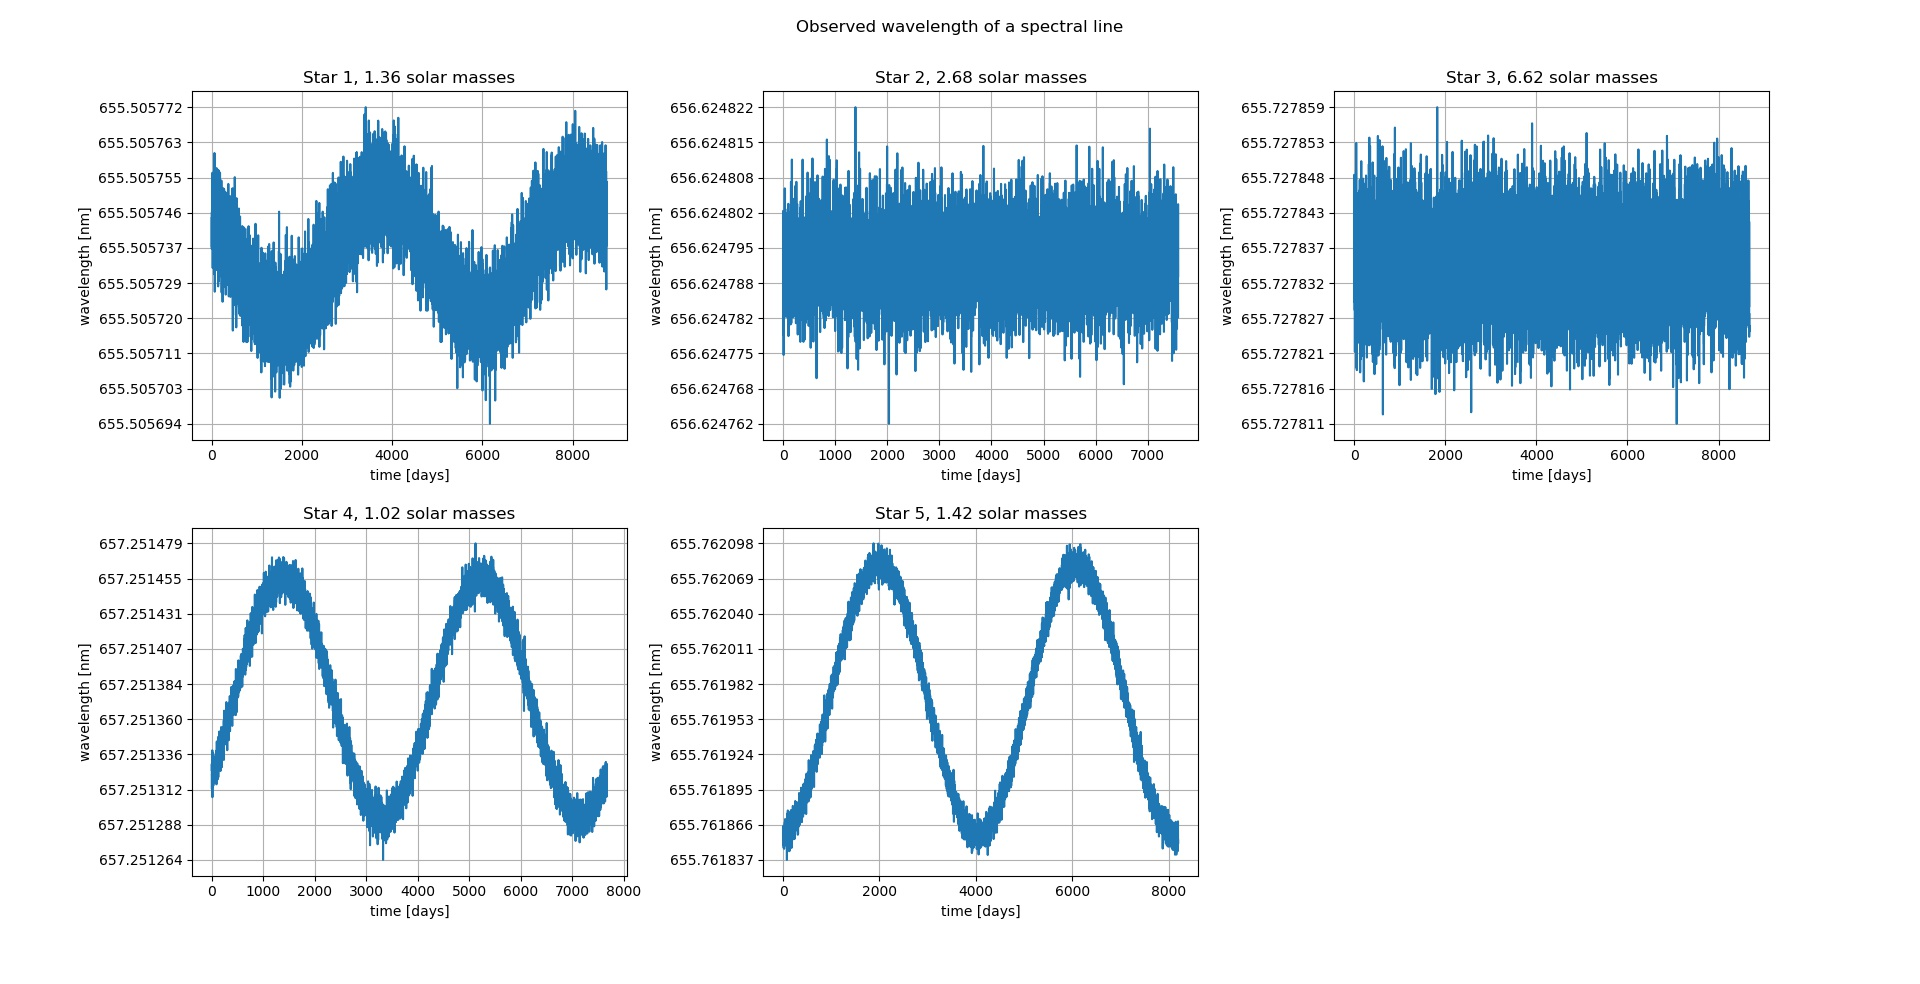
\includegraphics[width=\linewidth]{../output/plots/wavelengths_raw.jpg}
  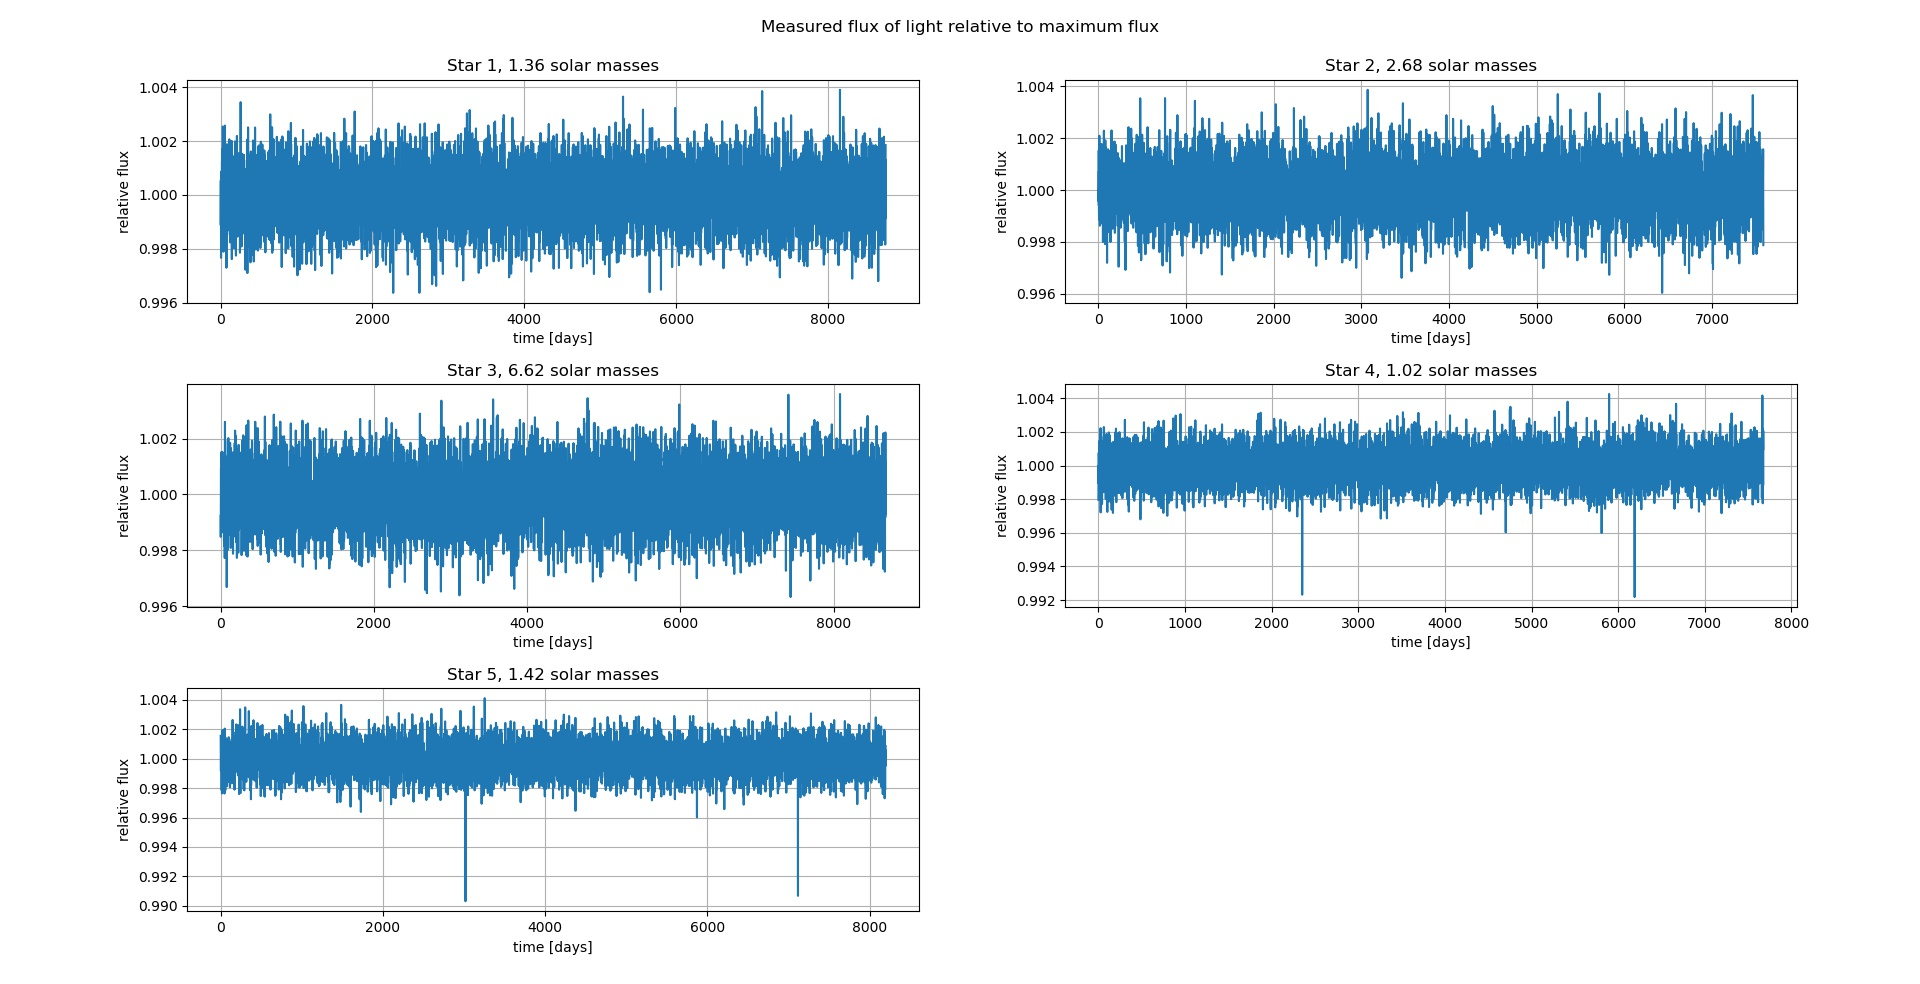
\includegraphics[width=\linewidth]{../output/plots/flux_raw.jpg}
  \caption{Illustrasjon av observert bølgelengde og relativ fluks for de fem stjernene.}
  \label{fig:raw_data}
\end{figure}

\begin{figure}
  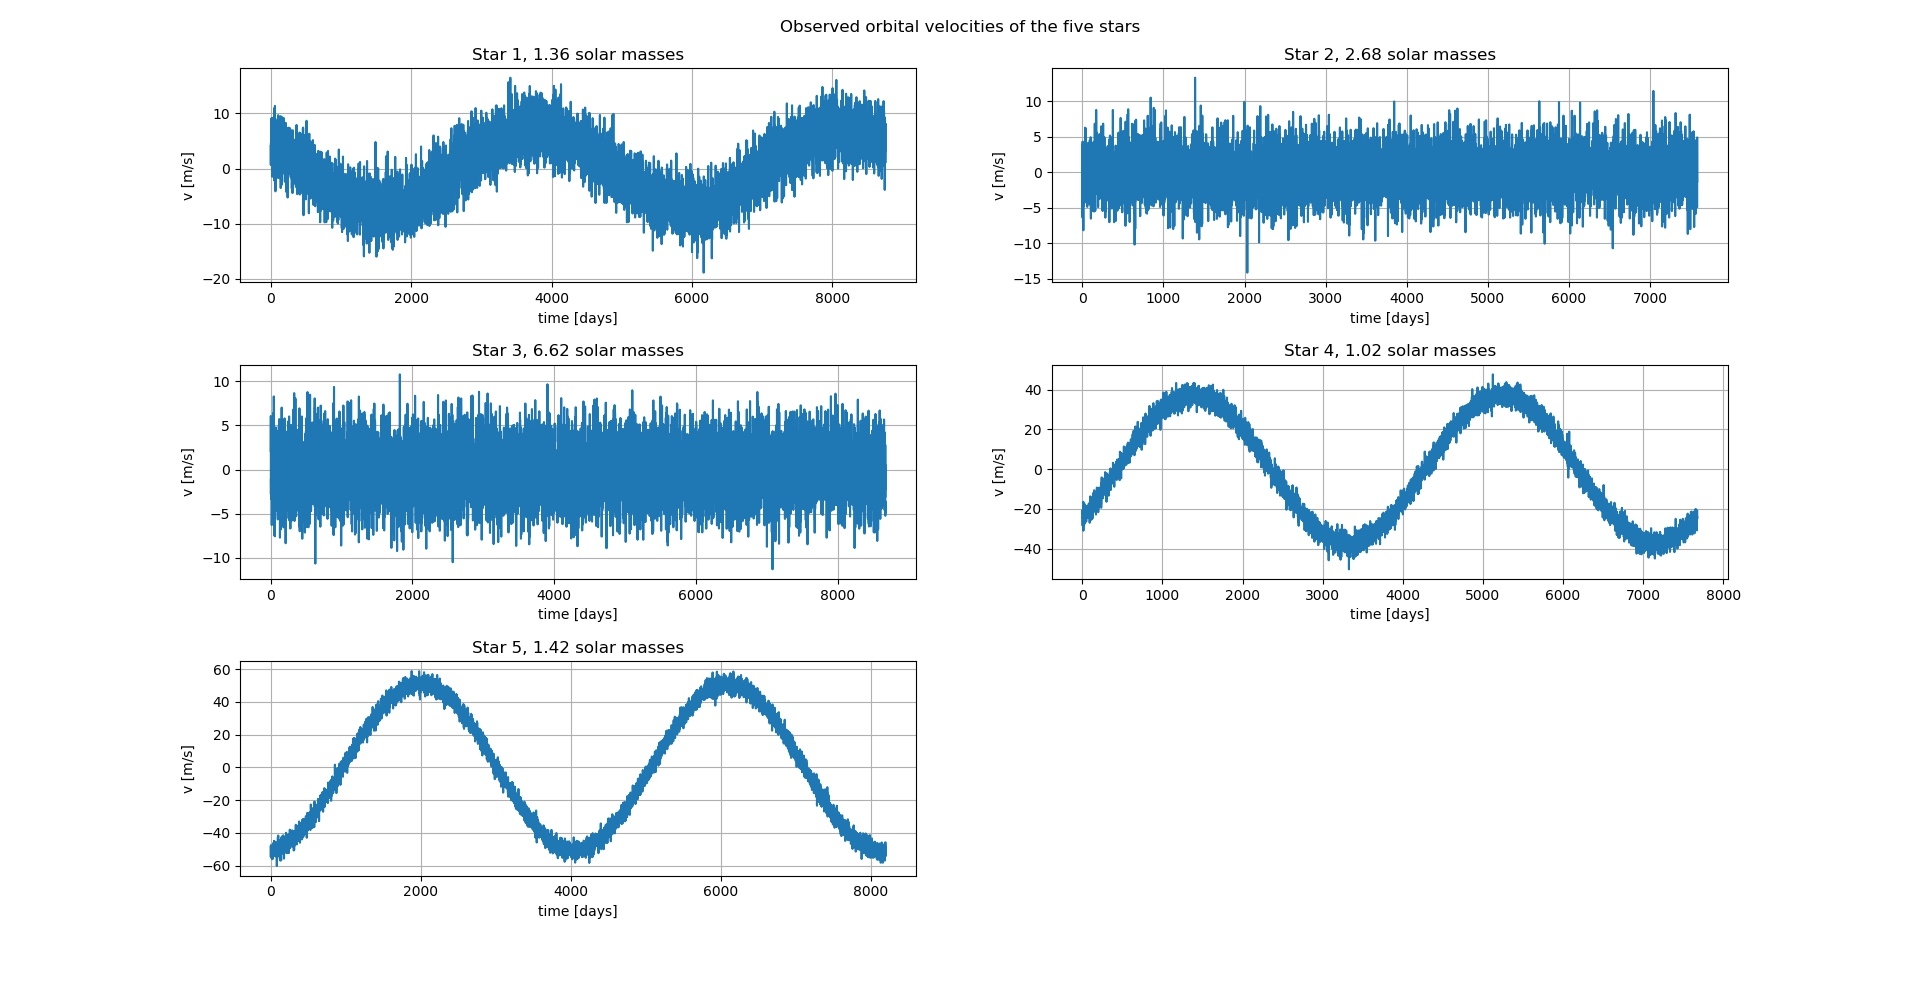
\includegraphics[width=\linewidth]{../output/plots/obs_orb_vels.jpg}
  \caption{Farten som vi observerer at stjernene har i sine baner.}
  \label{fig:obs_orb_vels}
\end{figure}

Figur \ref{fig:obs_orb_vels} viser hvilke hastigheter stjernene har parallelt med vår
 siktlinje i sine baner. For stjerne 1 kan vi lese av $v_{max} \approx 7$m/s og periode $P \approx 8000 - 3800 = 4200$ dager. For stjerne 4 får vi $v_{max} \approx 37$m/s og periode $P \approx 5200 - 1300 = 3900$ dager. For stjerne 5 får vi $v_{max} \approx 50$m/s og $P \approx 6100 - 2000 = 4100$ dager.

Ved å bruke likning \ref{eq:planet_mass} får jeg at minsteverdien for massene til
 planetene som går i bane rundt stjernene er:
 \begin{itemize}
  \item Stjerne 1: $1.30*10^{27}$kg
  \item Stjerne 4: $5.41*10^{27}$kg
  \item Stjerne 5: $9.44*10^{27}$kg
 \end{itemize}

Least squares metoden for å finne parametrene $v_r$, $P$ og $t_0$ gir resultatene som
 er listet under. Korresponderende verdier for den beregnede massen er også oppgitt. Figur \ref{fig:modelled_vel} viser hvordan den modellerte hastigheten passer sammen med måledataen vår.
\verbatiminput{../output/params_masses_precision.txt}

\begin{figure}
  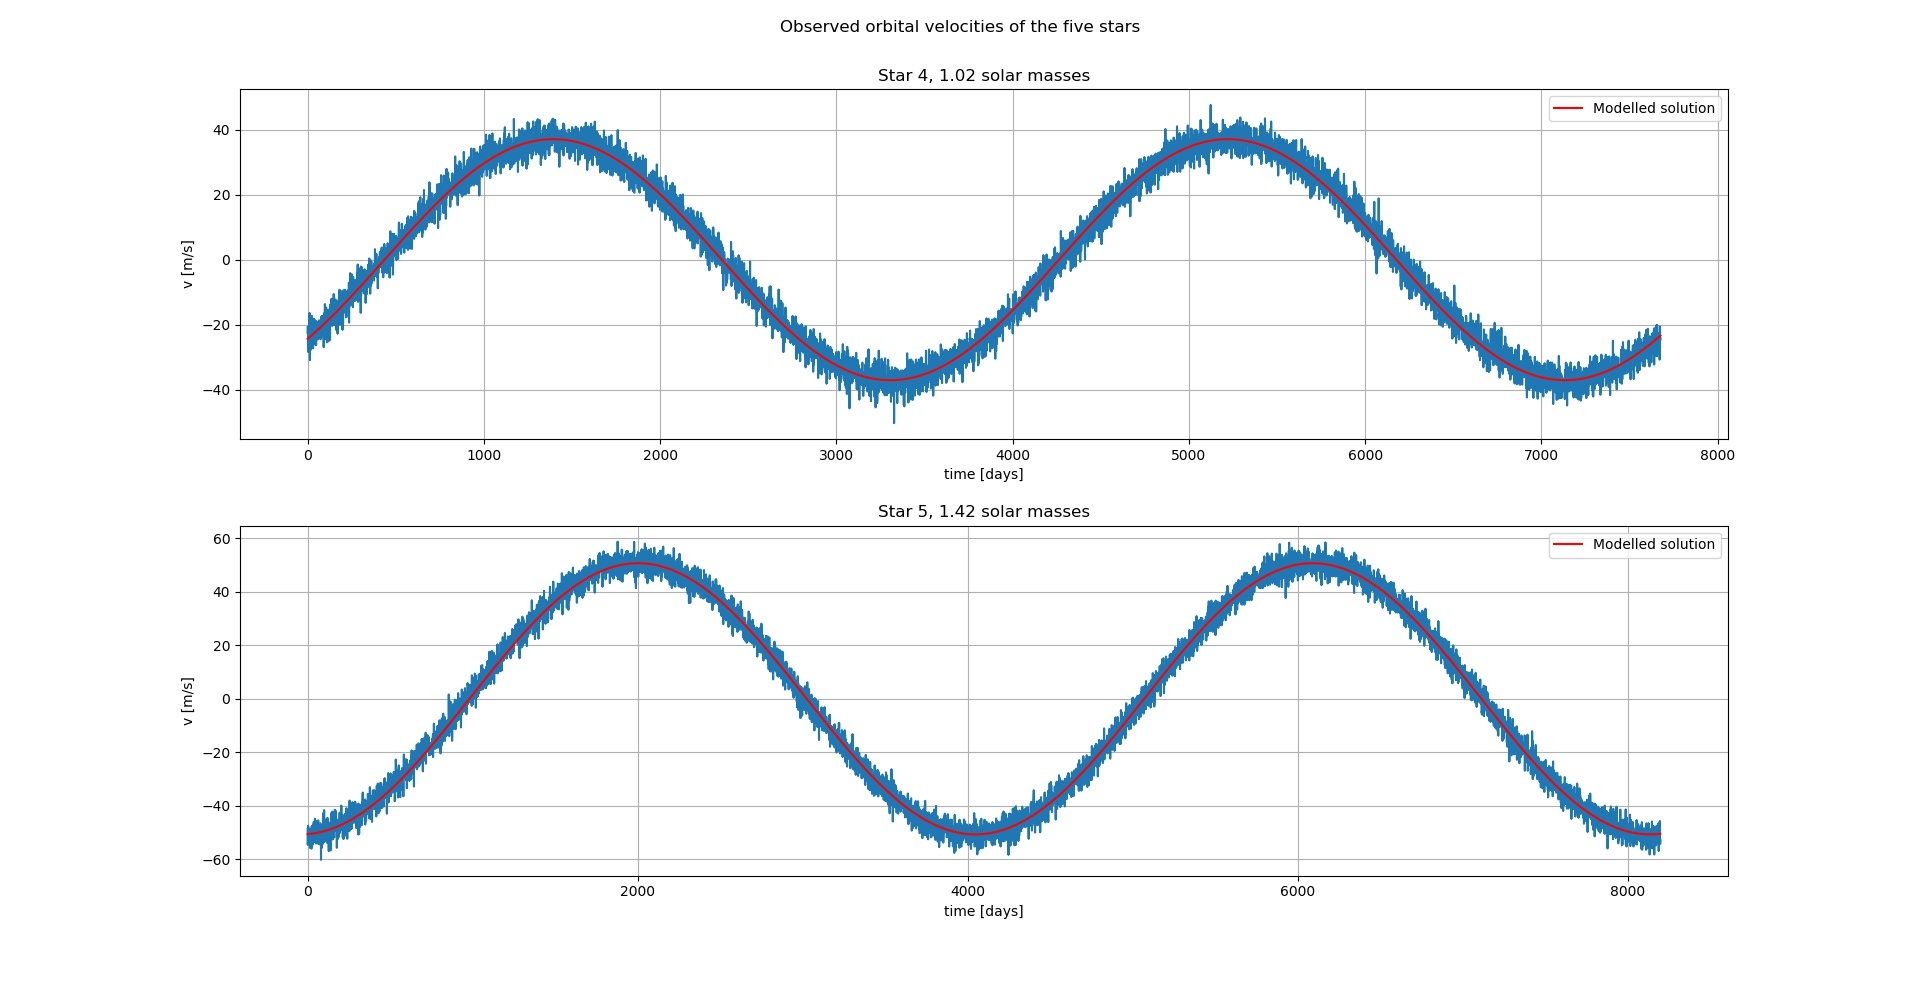
\includegraphics[width=\linewidth]{../output/plots/modelled_vel.jpg}
  \caption{Den modellerte hastigheten med verdiene for $v_r$, $P$ og $t_0$ fra least squares sammen med hastighetene vi får direkte fra måledataen.}
  \label{fig:modelled_vel}
\end{figure}



\section{Diskusjon}

Ved å se på figur \ref{fig:obs_orb_vels} ser vi tydelige periodiske svingninger i
 hastigheten til stjernene 1, 4 og 5. Det betyr at disse stjernene beveger seg i baner og
 har en komponent av banehastigheten som er parallell med vår siktlinje. For at stjernene skal gå i bane, må de påvirkes av en gravitasjonskraft som antakelig kommer fra en
 nærliggende planet. Det virker derfor som at stjernene 1, 4 og 5 har en planet i bane
 rundt seg. Vi kan ikke utelukke at stjerner 2 og 3 har planeter i bane rundt seg. Det
 eneste vi kan si er at de ikke går i bane med komponenter av banehastigheten som peker
 langs vår siktlinje. Dersom de går i baner hvis normalvektor er parallell med vår
 siktlinje vil lyset som når oss aldri bli rød- eller blåforskjøvet, og vi vil ikke se
 spor av banebevegelsen ved hjelp av denne teknikken.

Ved å studere illustrasjonen av fluks i figur \ref{fig:raw_data}, kan vi se at vi har to
 markante dropp i relativ flukstetthet for hver av stjernene 4 og 5. Disse droppene er i begge tilfeller med én periodes mellomrom. Dette tyder på at stjernene har hver sin planet som av og til passerer mellom jorda og stjerna. Dette stemmer også godt overens med at vi observerer størst variasjon i banefart for disse to stjernene. Disse resultatene sammen betyr at stjernene begever seg i baner der normalvektoren til banene står nært vinkelrett på vår siktlinje. Det betyr at den maksimale verdien for banefart vi observerer for stjernene er nær den virkelige banefarten til stjernene. Det betyr også at massen vi beregner ved å bruke likning \ref{eq:planet_mass} er nær den virklige massen til planeten da $\sin{i} \approx 1$.

Det viser seg at i den dataen vi har for fluks så er det ikke gjort målinger ofte nok
 til å kunne beregne radien til planetene som passerer foran stjernene 4 og 5. Vi kan heller ikke si noe om atmosfæren til planetene fordi vi bare måler fluksen til lys med én bølgelengde. Vi har bare rundt én måling per dag, og vi har kun utslag på fluksen som forteller oss at en planet er mellom oss og stjernen ved én av målingene for hver passering. Se figur \ref{fig:eclipse}. Vi kan altså ikke se akkurat når planeten begynner å bevege seg foran stjernen og tiden så snart hele planeten er foran stjernen, vi kan bare se ved én måling at hele planeten er foran stjernen. Ved mer frekvente målinger kunne vi beregnet radien til planeten, og evt størrelse og innhold til atmosfæren.

\begin{figure}
  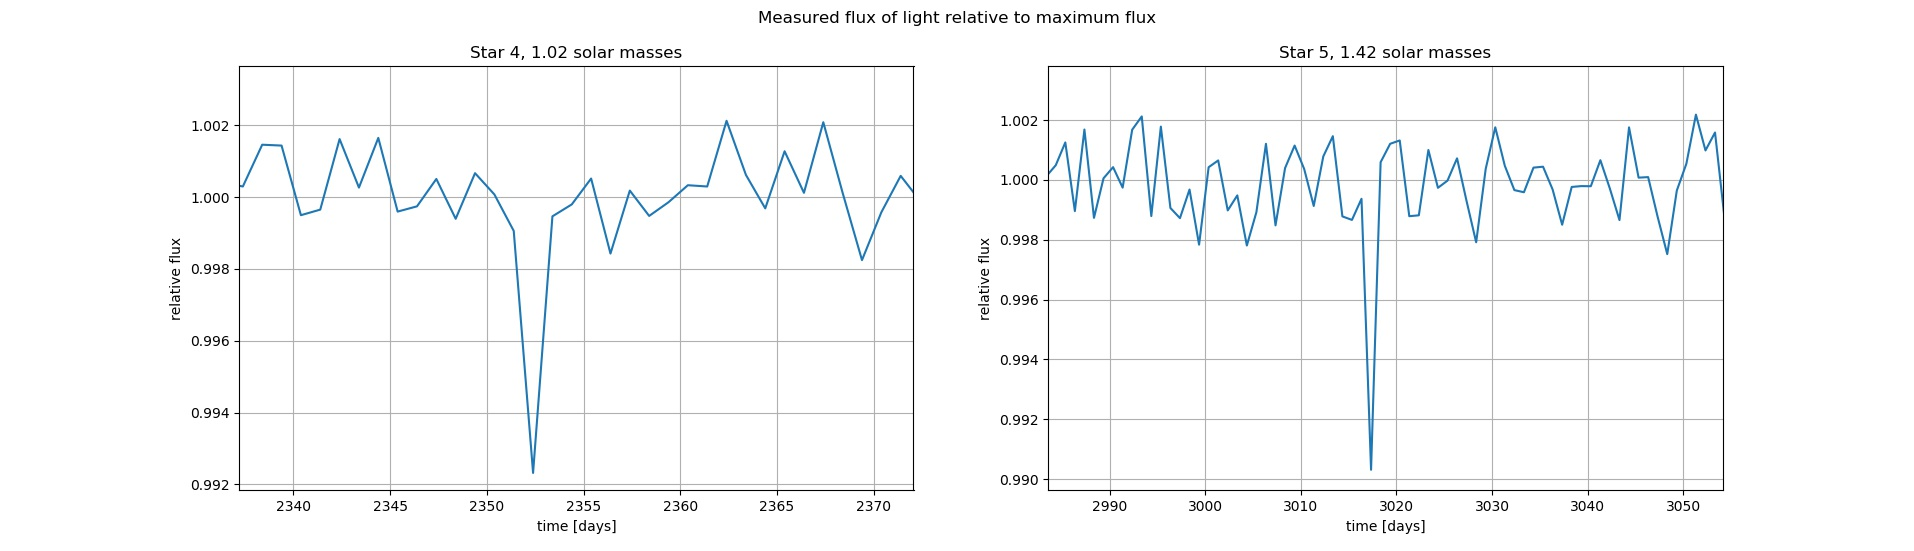
\includegraphics[width=\linewidth]{../output/plots/eclipse.jpg}
  \caption{Nærbilde av illustrasjonen for den relative fluksen når en planet passerer foran stjernen. Man ser at vi bare har én måling for hver gang planeten er foran stjernen.}
  \label{fig:eclipse}
\end{figure}

For å finne de beste verdiene for de frie parametrene i $v_r^{model}$ ved hjelp av least
 squares, velger jeg å teste med 40 verdier innenfor intervallet for hver parameter. Å øke antall testverdier vil selvsagt kunne gi bedre tilnærming, men vil også øke tiden det tar å utføre alle beregningene betraktelig. Å øke fra 30 til 40 testverdier på hver av parameterne gjør at den minste summen av kvadratavvikene reduseres med 1.4\% og 1.6\% for henholdsvis stjerner 4 og 5. Dette gjør at den beregnede massen endres med rundt 0.3\% for begge. Er det behov for større presisjon kan vi øke antall testverdier, og eventuelt finjustere grensene manuelt ved hjelp av de resultatene vi allerede har fått. Jeg velger 40 verdier ford jeg mener det er en god balanse mellom tiden det tar å kjøre beregningene og presisjonen som kreves. Vi har nå fått et ganske godt estimat på stjernenes bevegelse og massene til planetene.

\begin{thebibliography}{}
\bibitem[Hansen (2017)]{part1C} Hansen, F. K.,  2017, Forelesningsnotat 1C i kurset AST2000


\end{thebibliography}



\end{document}
